\documentclass[conference]{IEEEtran}
\IEEEoverridecommandlockouts
% The preceding line is only needed to identify funding in the first footnote. If that is unneeded, please comment it out.
\usepackage{cite}
\usepackage{amsmath,amssymb,amsfonts}
\usepackage{algorithmic}
\usepackage{graphicx}
\usepackage{textcomp}
\usepackage{hyperref}
\usepackage{xcolor}
\usepackage{tabulary}
\def\BibTeX{{\rm B\kern-.05em{\sc i\kern-.025em b}\kern-.08em
    T\kern-.1667em\lower.7ex\hbox{E}\kern-.125emX}}
\begin{document}

\title{The Observatory}

\author{\IEEEauthorblockN{1\textsuperscript{st} Fabio Plunser}
      \and
      \IEEEauthorblockN{2\textsuperscript{nd} Dominik Barbist}
      \and
      \IEEEauthorblockN{3\textsuperscript{rd} Florian Gruber}
}

\maketitle

\begin{quote}
\textit{"What is it worth to have hundreds of cameras if you can't spy on someone."}\\
--- The Observatory Team, 2024
\end{quote}

\section{Introduction}
For this project, we have implemented a system that can detect and track people across multiple cameras while identifying unknown faces.
The system processes video streams on the edge using YOLOv8 for person detection and implements a cross-camera tracking system.
When an unrecognized face is detected, it is sent to AWS Rekognition for comparison against known faces stored in S3.
If an unknown face is detected, the system triggers an alarm on the corresponding IoT device.
The system requires significant parallel processing capabilities to handle multiple video streams simultaneously.
\\
\textbf{Main Steps:}
\begin{itemize}
      \item \textbf{Data Collection:} Collection of video streams from both emulated and physical cameras (ESP32-CAM/Webcam) using WebSockets.
      \item \textbf{Data Processing:} Real-time person detection and tracking using YOLOv8 on the edge device.
      \item \textbf{Data Storage:} Company-isolated storage in AWS S3 for face images and SQLite for local state management.
      \item \textbf{Data Analysis:} Face comparison using AWS Rekognition with known faces database.
      \item \textbf{Signal Processing:} NATS-based messaging system for edge-cloud communication and WebSockets for device communication.
      \item \textbf{User Interface:} Real-time monitoring and control through a Svelte-based web interface.
\end{itemize}

\section{System architecture}
\begin{itemize}
      \item \textbf{Data Collection:} Multiple video streams are collected from both emulated cameras, ESP32-CAM devices, and webcams.
            Devices automatically discover the edge server using mDNS and establish WebSocket connections for streaming.          
      \item \textbf{Data Processing:} The edge server uses multiprocessing to handle multiple video streams concurrently.
            Each stream is processed using YOLOv8 for person detection, with hardware acceleration where available.
            A cross-camera tracking system maintains person identity across multiple views.          
      \item \textbf{Data Storage:} AWS S3 implements a company-centric structure with separate directories for known and unknown faces.
            The edge server maintains a SQLite database for device management, room organization, and face detection tracking.        
      \item \textbf{Data Analysis:} AWS Rekognition compares detected faces against the known faces database using the CompareFaces API.
            The edge server implements intelligent face detection to minimize cloud processing costs.       
      \item \textbf{Signal Processing:} NATS handles all edge-cloud communication including bucket management, URL generation,
            and face recognition requests. Device communication uses WebSockets with automatic reconnection capabilities.        
      \item \textbf{User Interface:} A Svelte-based web interface provides real-time camera monitoring, alarm management,
            and system configuration. The interface supports room-based organization and device management.
\end{itemize}
% Describe your system in detail, including a figure for your architectural diagram (IoT, Edge, Cloud layers, components developed and services used).

\begin{figure}[h!]
      \centering
      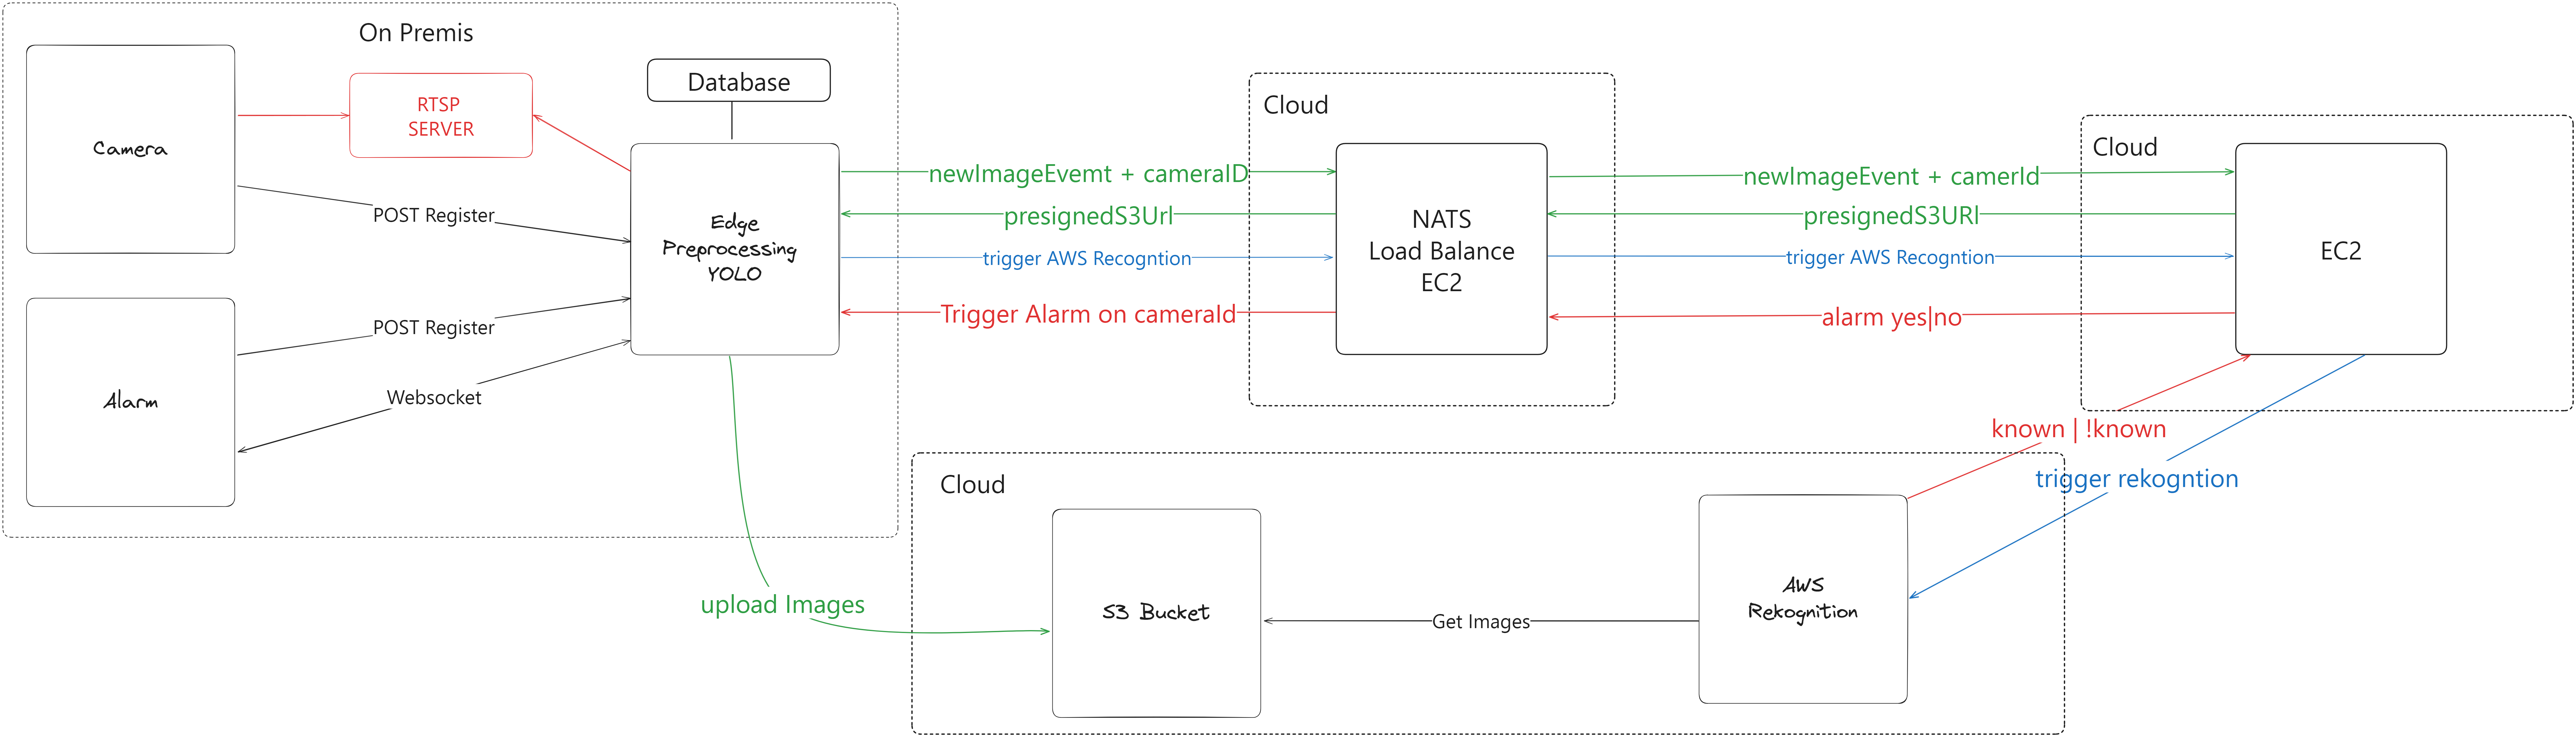
\includegraphics[width=1\linewidth]{images/architecturev2.excalidraw.png}
      \caption{Prototype of the system architecture.}
      \label{fig:enter-label}
\end{figure}

\section{Implementation details}
\subsection{System Components}
\begin{itemize}
      \item \textbf{Video Input Sources:} 
            \begin{itemize}
                  \item RTSP stream support for IP cameras
                  \item OpenCV-based camera emulation
                  \item ESP32-CAM integration
                  \item Base64/WebSocket fallback protocol
                  \item WiseNet dataset integration
                  \item Automatic stream recovery
            \end{itemize}

      \item \textbf{Edge Server Core:} 
            \begin{itemize}
                  \item Python-based async server architecture
                  \item RTSP stream handling with FFmpeg
                  \item mDNS service registration
                  \item SQLite with SQLAlchemy for some persistence
            \end{itemize}
      \item \textbf{Camera Implementation:} 
            \begin{itemize}
                  \item Primary RTSP stream support for all cameras
                  \item OpenCV-based frame processing pipeline
                  \item ESP32-CAM integration with RTSP streaming
                  \item WebSocket streaming for web interface display
                  \item Automatic stream recovery and reconnection
                  \item Configurable frame rate and quality settings(only in code not in the web interface)
            \end{itemize}
      \item \textbf{Development Dataset:} 
            \begin{itemize}
                  \item Integration of WiseNet surveillance dataset
                  \item 6 camera feeds with 11 video sequences each
                  \item Automatic sequence looping for continuous testing
                  \item Configurable frame rates and resolutions(only in code not in the web interface)
            \end{itemize}
      \item \textbf{Web Interface:} 
            \begin{itemize}
                  \item Svelte-based reactive frontend
                  \item Real-time video stream display using WebSockets
                  \item Person tracking visualization overlay
                  \item Device management interface
                  \item Alarm control and monitoring
                  \item Cloud connection configuration
            \end{itemize}
\end{itemize}
\subsection{Data Processing}
\begin{itemize}
      \item \textbf{Stream Processing:} The system processes RTSP streams using FFmpeg and OpenCV for efficient video decoding.
            Multiple video streams are handled concurrently through multiprocessing to maximize system resources.
            The processor implements frame skipping to lighten the processing load while maintaining effective detection rates.
            and includes automatic reconnection capabilities to handle temporary stream disruptions.
      \item \textbf{Video Processing:} The edge server handles multiple video streams concurrently using Python's multiprocessing. 
            Each camera stream is processed in separate processes to maximize CPU utilization. The video processor implements frame skipping 
            to reduce processing load while maintaining effective detection rates.
      \item \textbf{YOLO:} For face detection and person detection we use YOLOv8n, the most lightweight model of the YOLOv8 family. 
            The model runs on the edge server and processes each camera feed in real-time. We utilize hardware acceleration where available,
            supporting CUDA for NVIDIA GPUs and MPS for Apple Silicon, with CPU fallback.
      \item \textbf{Tracking:} We implement multi-camera person tracking using ByteTrack for real-time person tracking and using torchreid for the person re-identification task. 
            This allows us to maintain person identity across multiple camera views and avoid redundant face recognition requests. 
            Each tracked person maintains their recognition status (pending, in\_progress, recognized, unknown) and face ID across the system.
\end{itemize}

\subsection{Data Storage}
\begin{itemize}
      \item \textbf{AWS S3:} Our storage solution utilizes a single S3 bucket named 'the-observatory-faces' that implements 
            a company-centric organizational structure for comprehensive face management. The bucket's root level contains 
            individual folders for each company using our system. Within each company folder, we maintain two distinct directories: 
            'known-faces' and 'unknown-faces'. The 'known-faces' directory stores pre-approved facial records of employees and 
            authorized personnel, while 'unknown-faces' automatically accumulates detected faces that don't match any known records.
      \item \textbf{Database:} The edge server uses SQLite with SQLAlchemy for local data management. The schema includes:
            \begin{itemize}
                  \item Company settings and cloud connection details
                  \item Camera and alarm device management
                  \item Room-based organization of devices
                  \item Face detection tracking and temporary storage
            \end{itemize}
\end{itemize}

\subsection{Data Analysis}
\begin{itemize}
      \item \textbf{Amazon Rekognition:} We use AWS Rekognition's CompareFaces API to match detected faces against the known faces
            database. If a face is not recognized, the system triggers an alarm on the corresponding IoT device.
      \item \textbf{Edge Processing:} The edge server performs initial face detection and tracking locally, only sending faces to
            the cloud when necessary. This hybrid approach reduces cloud costs and network bandwidth while maintaining quick response times.
\end{itemize}

\subsection{Signal Processing}
\begin{itemize}
      \item \textbf{NATS Messaging:} We use NATS for all edge-to-cloud communication. The system implements:
            \begin{itemize}
                  \item Bucket initialization and management commands
                  \item Presigned URL generation for S3 uploads/downloads
                  \item Face recognition execution requests
                  \item Alarm trigger notifications
            \end{itemize}
      \item \textbf{Device Communication:} Devices discover the edge server using mDNS (Zeroconf). Video streams and alarm
            status updates are handled through WebSocket connections, with fallback mechanisms for connection recovery.
\end{itemize}

\subsection{User Interface}
\begin{itemize}
      \item \textbf{Web Application Features:}
            \begin{itemize}
                  \item Centralized surveillance dashboard
                  \item Multi-camera live view with person tracking overlay
                  \item Known face management and upload interface
                  \item Alarm status monitoring and control panel
                  \item Company-wide system configuration
                  \item Cloud connection management interface
            \end{itemize}
      
      \item \textbf{Technical Implementation:} 
            \begin{itemize}
                  \item Static Svelte application for optimal performance
                  \item Real-time WebSocket communication
                  \item Responsive design for various screen sizes
                  \item Client-side face image preprocessing
                  \item Automatic connection recovery
                  \item Session persistence
            \end{itemize}

      \item \textbf{Security Features:} 
            \begin{itemize}
                  \item Company-isolated data access
                  \item Secure WebSocket connections
                  \item Presigned URL-based cloud storage access
                  \item Automatic session management
            \end{itemize}
\end{itemize}

\section{Evaluation}
\label{sec:evaluation}
Sadly this section is still incomplete and will be updated in the final report.
Our evaluation focuses on three key aspects:

\begin{itemize}
      \item \textbf{Processing Performance:} 
            \begin{itemize}
	\item Successfully processed multiple video streams concurrently(6 cameras + 1 Webcam), but at this but the frame rate is not optimal.
	\item Detect new people in less than 2 seconds  
		\item Successfully processed multiple video streams concurrently(6 cameras + 1 Webcam), but at this but the frame rate is not optimal.
	\item Detect new people in less than 2 seconds  
\end{itemize}

\item \textbf{Scalability:}
\begin{itemize}
	\item Connecting additional cameras should be straightforward
	\item The Nats messaging system allows for easy scaling of the system
\end{itemize}
\item \textbf{Reliability:}
\begin{itemize}
	\item Automatic stream recovery and reconnection
	\item Start scripts for easy deployment on new devices
\end{itemize}
\end{itemize}
\subsection{Measurements}
\begin{itemize}
	\item 24 Images and 5 parallel:
	\begin{table}[h]
		\begin{tabulary}{\textwidth}{|C|C|C|C|C|}
			\hline
			\textbf{Name} &
			\textbf{min.} &
			\textbf{max.} &
			\textbf{mean} &
			\textbf{median} 
			\\\hline
			Total processing time & 0.675 & 1.360 & 0.869 & 0.794  \\\hline
			Presigned url request time & 0.120 & 0.194 & 0.143 & 0.133  \\\hline
			Image upload time & 0.499 & 1.161 & 0.720 & 0.657  \\\hline
			Recognition time & 0.000 & 0.000 & 0.000 & 0.000 \\\hline
		\end{tabulary} 
	\end{table}
	
	\item 	 24 Images and 24 parallel:
	\begin{table}[h]
		\begin{tabulary}{\textwidth}{|C|C|C|C|C|}
			\hline
			\textbf{Name} &
			\textbf{min.} &
			\textbf{max.} &
			\textbf{mean} &
			\textbf{median}
			\\\hline
			Total processing time & 0.087 & 1.648 & 1.224 & 1.189  \\\hline
			Presigned url request time & 0.214 & 0.349 & 0.266 & 0.270  \\\hline
			Image upload time & 0.609 & 1.372 & 0.954 & 0.933  \\\hline
			Recognition time & 0.000 & 0.000 & 0.000 & 0.000 \\\hline
		\end{tabulary} 
	\end{table}
	
	
	\item 	 100 Images and 100 parallel:
	\begin{table}[h]
		\begin{tabulary}{\textwidth}{|C|C|C|C|C|}
			\hline
			\textbf{Name} &
			\textbf{min.} &
			\textbf{max.} &
			\textbf{mean} &
			\textbf{median} 
			\\\hline
			Total processing time & 1.162 & 8.845 & 5.962 & 7.779  \\\hline
			Presigned url request time & 0.509 & 1.659 & 1.089 & 1.061  \\\hline
			Image upload time & 0.588 & 7.720 & 4.869 & 6.447  \\\hline
			Recognition time & 0.000 & 0.000 & 0.000 & 0.000 \\\hline
		\end{tabulary} 
	\end{table}
	\item 	 200 Images and 200 parallel:
	\begin{table}[h]
		\begin{tabulary}{\textwidth}{|C|C|C|C|C|}
			\hline
			\textbf{Name} &
			\textbf{min.} &
			\textbf{max.} &
			\textbf{mean} &
			\textbf{median} 

			\\\hline
			Total processing time & 1.487 & 8.254 & 5.370 & 5.580  \\\hline
			Presigned url request time & 0.820 & 2.920 & 1.354 & 1.046 \\\hline
			Image upload time & 0.649 & 6.426 & 4.012 & 4.507  \\\hline
			Recognition time & 0.000 & 0.000 & 0.000 & 0.000 \\\hline
		\end{tabulary} 
	\end{table}
\end{itemize}
\subsection{Performance Analysis Graphs}

\subsubsection{Total Processing Time Analysis}
The total processing time analysis reveals comprehensive system performance characteristics across different parallel processing configurations. The minimum processing times show a relatively modest increase from 0.675 seconds with 5 parallel processes to 1.487 seconds with 200 parallel processes, demonstrating good baseline scalability. The maximum processing times exhibit more dramatic scaling effects, peaking at approximately 8.8 seconds for the 100-parallel configuration and showing slightly better performance at 8.2 seconds for the 200-parallel configuration, which suggests potential optimization in resource utilization at higher scales. The mean processing times demonstrate a significant jump when moving from 24 parallel processes (1.224 seconds) to 100 parallel processes (5.962 seconds), indicating a potential performance threshold where resource contention becomes a limiting factor. The median values closely follow the mean times but show some deviation in the 100-parallel configuration, suggesting occasional performance outliers that affect the average. The overall trend indicates that while the system can handle increased parallelism, there are clear performance trade-offs beyond certain thresholds, particularly when processing more than 24 concurrent requests.
\begin{figure}[h]	
	\centering
	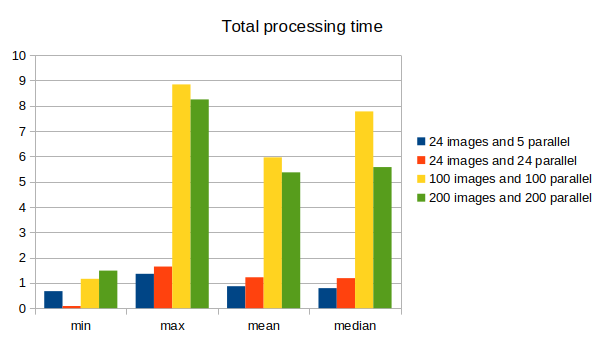
\includegraphics[width=6cm,height=6cm,keepaspectratio]{images/measurements_cloud/total_processing_time.png}
	\caption{Total processing time.}
	\label{total-processing-time}
\end{figure}
\subsubsection{Image Upload Time Analysis}
The image upload time graph demonstrates a clear correlation between parallel processing load and upload duration, with the 100-parallel and 200-parallel configurations showing significantly higher maximum upload times of approximately 7.7 and 6.4 seconds respectively. The minimum upload times remain relatively consistent across all configurations, ranging from 0.5 to 0.7 seconds, suggesting a baseline network overhead regardless of parallel load. The mean upload times show a notable increase from around 0.7 seconds with 24 images to approximately 4.5 seconds with larger batches, indicating potential resource contention or network bandwidth limitations at higher scales. Interestingly, the 200-parallel configuration shows slightly better performance than the 100-parallel configuration in terms of median upload time, suggesting possible optimization in the connection pooling or resource allocation at larger scales. The relatively small difference between mean and median values in the 24-image configurations indicates a more predictable performance at lower parallel loads, while the larger spreads in the 100 and 200 image configurations suggest more variable performance under heavy load.
\begin{figure}[h]	
	\centering
	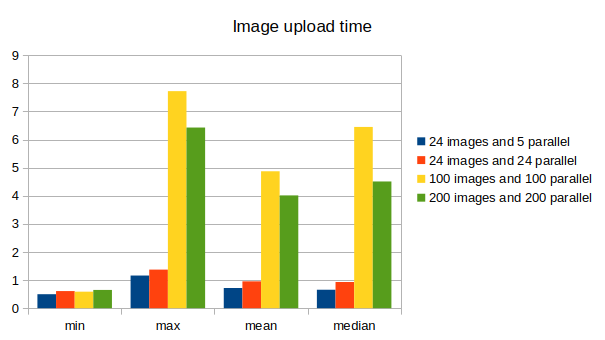
\includegraphics[width=6cm,height=6cm,keepaspectratio]{images/measurements_cloud/image_upload_time.png}
	\caption{Image upload time.}
	\label{image-upload-time}
\end{figure}

\subsubsection{Presigned URL Request Time Analysis}
The presigned URL request time analysis reveals a clear scaling pattern, with request times increasing proportionally with the number of parallel operations. The minimum request times show a gradual increase from 0.12 seconds with 5 parallel requests to 0.82 seconds with 200 parallel requests, indicating growing overhead in the AWS authentication and URL generation system. The maximum request times demonstrate more pronounced scaling effects, reaching nearly 3 seconds for the 200-parallel configuration, which suggests potential bottlenecks in the URL generation service under high concurrent loads. The mean request times maintain a relatively linear relationship with the number of parallel requests, increasing from 0.143 seconds to 1.354 seconds as parallelism scales up. The median values closely track the means in most configurations, indicating a fairly normal distribution of request times without significant outliers. Most notably, the spread between minimum and maximum times widens considerably at higher parallelism, suggesting decreased predictability in request latency under heavy load.
\begin{figure}[h]	
	\centering
	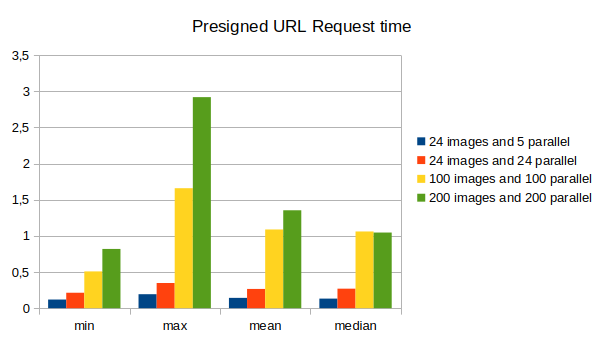
\includegraphics[width=6cm,height=6cm,keepaspectratio]{images/measurements_cloud/presigned_url_request_time.png}
	\caption{Presigned URL request time.}
	\label{presigned-url-request-time}
\end{figure}


\end{document}
